\chapter{Theoretische Grundlagen}
\label{chap:theoretische_grundlagen}
\section{Greensche Funktionen}
Die Greensche Funktion ist für zwei beliebige Operatoren $A$ und $B$ mit der zeitlichen Entwicklung 
\begin{equation}
    A \left ( \tau \right ) = \symup{e}^{H \tau} A_\text{S} \symup{e}^{-H \tau}  \label{eqn:heisenbergpic}, 
    \quad B \left ( \tau' \right ) = \symup{e}^{H \tau'} B_\text{S} \symup{e}^{-H \tau'}
\end{equation}
definiert als 
\begin{align}
    G_{A,B} \left (\tau, \tau' \right ) &= - \frac{1}{\hbar} \langle T_s \left ( A \left (\tau \right ) B \left ( \tau' \right ) \right ) \rangle \\
    & = - \frac{1}{\hbar} \left(  \langle A \left (\tau \right ) B \left ( \tau' \right ) \rangle \symup{\Theta} \left ( \tau - \tau' \right) + s 
    \langle B \left ( \tau' \right ) A \left (\tau \right ) \rangle \symup{\Theta} \left ( \tau' - \tau \right)  \right ) \; \text{,} \label{eqn:greensfunction}
\end{align}
wobei $\tau = \symup{i}t$ eine komplexwertige Zeit und $t$ die gewöhnliche, reelle Zeit, $H$ der Hamiltonoperator, $A_\text{S}$ ein Operator im Schöringerbild, $T_s$ der Zeitordnungsoperator, 
$\langle \ldots \rangle$ ein Erwartungswert und $\symup{\Theta} \left ( \tau' - \tau \right)$ die Heaviside-Funktion ist \cite{greensfunction}.
Der Parameter $s$ sorgt mit $s=+1$ für bosonische bzw. $s=-1$ für fermionische Operatoren für das richtige Vorzeichen.
Der Erwartungswert eines Operators $A$ ist bezüglich der großkanonischen Gesamtheit durch 
\begin{equation*}
    \langle A \rangle = \frac{1}{Z} \text{Sp}(\symup{e}^{-\beta H} A)
\end{equation*}
gegeben \cite{greensfunction}.
Die Zustandssumme $Z$ stellt dabei einen Normierungsfaktor dar.
In Gleichung \eqref{eqn:heisenbergpic} wurde das reduzierte Planksche Wirkungsquantum $\hbar$ bereits auf eins gesetzt, was in den folgenden Abschnitten beibehalten wird.
Da in dieser Arbeit nur fermionische Systeme betrachtet werden, wird $s$ ab jetzt ohne weitere Bemerkungen auf $-1$ gesetzt.
Die zeitliche Entwicklung eines Opertators $A (\tau)$ ist gemäß der Differentialgleichung 
\begin{equation}
\frac{\partial}{\partial t} A \left (\tau \right ) = \symup{i}  [H, A] \iff \frac{\partial}{\partial \tau} A \left (\tau \right ) = [H, A] \label{eqn:heisenbergeom}
\end{equation}
festgelegt.
Für die hier behandelte Modellierung ist die Bewegungsgleichung für die Greensche Funktion \eqref{eqn:greensfunction} von großer Bedeutung, welche mittels 
partieller Ableitung nach der Zeit gewonnen werden kann \cite{greensfunction}.
Somit folgt
\begin{align*}
    \frac{\partial}{\partial \tau} G_{A,B} \left (\tau, \tau' \right) = 
    &- \left \langle \frac{\partial}{\partial \tau}A \left (\tau \right ) B \left ( \tau' \right ) \right \rangle
    \symup{\Theta} \left ( \tau - \tau' \right) -  \langle A \left (\tau \right ) B \left ( \tau' \right ) \rangle \delta \left ( \tau - \tau' \right)\\
    &+ \left \langle B \left ( \tau' \right ) \frac{\partial}{\partial \tau}A \left (\tau \right ) \right \rangle \symup{\Theta} \left ( \tau' - \tau \right)
    -  \langle B \left ( \tau' \right ) A \left (\tau \right ) \rangle \delta \left ( \tau' - \tau \right)
    \\[2ex]
    = &- \left \langle [H,A] B \left ( \tau' \right ) \right \rangle
    \symup{\Theta} \left ( \tau - \tau' \right) -  \langle A \left (\tau \right ) B \left ( \tau' \right ) \rangle \delta \left ( \tau - \tau' \right)\\
    &+ \left \langle B \left ( \tau' \right ) [H,A] \right \rangle \symup{\Theta} \left ( \tau' - \tau \right)
    -  \langle B \left ( \tau' \right ) A \left (\tau \right ) \rangle \delta \left ( \tau' - \tau \right)
    \\[2ex]
    =\; & G_{[H,A],B}(\tau, \tau') - \langle \{ A,B \} \rangle \delta \left ( \tau - \tau' \right) \; \text{.} \numberthis \label{eqn:eomgreen}
\end{align*} 
Dabei ist  $\delta (\tau-\tau') = \delta (\tau'-\tau) $ die Deltadistribution als Ableitung der Heaviside-Funktion und 
$\{ A,B \} = AB+BA$ der Antikommutator.
In der dritten Zeile wurde Gleichung \eqref{eqn:heisenbergeom} ausgenutzt.
Um algebraisch anstatt mit Differentialen rechnen zu können, wird die Bewegungsgleichung \eqref{eqn:eomgreen} fouriertransformiert,
womit sich
\begin{equation}
    zG_{A,B}(z) = \langle \{A,B\} \rangle - G_{[H,A],B}(z) \label{eqn:fouriereom}
\end{equation} 
ergibt \cite{anders-fkt}.
Die Variable $z$ ist eine komplexwertige Frequenz.
Eine wichtige Eigenschaft der Greenschen Funktion ist die Linearität, aus welcher mit $\alpha, \beta \in \mathbb{C}$
\begin{equation*}
    G_{(\alpha A + \beta B), C} = \alpha G_{A,C} + \beta G_{B,C}
\end{equation*}
folgt.
\section{Tight Binding Modell}
\label{sec:tightbinding}
In der Tight Binding Näherung wird von stark gebundenen, lokalisierten Elektronen ausgegangen \cite{Czycholl}.
Dazu wird der volle Hamiltonian eines Elektrons im Festkörper
\begin{equation}
    H = \frac{\vec{p}^2}{2M} + \sum_{j\alpha} v(\vec{r}-\vec{l}_j - \vec{R}_{\alpha}) = \frac{\vec{p}^2}{2M} + v_{\vec{R}}(\vec{r})\label{eqn:electron_hamiltonian}
\end{equation}
betrachtet \cite{Czycholl}.
Der Vektor $\vec{R}_{\alpha}$ ist die Position der Atome innerhalb der Einheitszelle mit dem Gittervektor $\vec{l}_j$, während
$\vec{p} = -\symup{i}\vec{\nabla}$ der Impulsoperator, $M$ die Masse des Elektrons und $v_{\vec{R}}(\vec{r})$ mit $\vec{r}$ als Ortsvektor das Potential von den Atomen in dem Festkörper, 
was auf das betrachtete Elektron wirkt, ist.
Mittels des Wellenvektors $\vec{k}$ lassen sich aus den lokalen atomaren Wellenfunktionen $\Psi_{lm} \left (\vec{r}-\vec{l}_j - \vec{R}_{\alpha} \right )$ mit $l$ und $m$ als lokale Drehimpulsquantenzahlen
Blochzustände
\begin{equation}
    \Psi^{\alpha}_{lm}(\vec{k}, \vec{r}) = \frac{1}{\sqrt{N}} \sum_{j} \symup{e}^{\symup{i}\vec{k}\vec{l}_j} \Psi_{lm}(\vec{r}-\vec{l}_j - \vec{R}_{\alpha}) 
\end{equation}
konstruieren, welche die Gitterperiodizität besitzen \cite{SC_literature}.
Für die Tight Binding Modellierung werden die Matrixelemente des Hamiltonians \eqref{eqn:electron_hamiltonian}
benötigt, welche sich in der Blochbasis durch
\begin{equation*}
    \bra{\Psi^{\alpha}_{lm}(\vec{k})} H \ket{\Psi^{\alpha'}_{l'm'}(\vec{k})} = \varepsilon_{lm,l'm'}^{\alpha \alpha'} \braket*{\Psi^{\alpha}_{lm}(\vec{k})}{\Psi^{\alpha'}_{l'm'}(\vec{k})}
    - \frac{1}{N} \sum_{j\alpha \neq j' \alpha'} \symup{e}^{\symup{i}\vec{k}(\vec{l}_{j'}-\vec{l}_{j})}  t^{j\alpha,j'\alpha'}_{lm,l'm'}
\end{equation*}
errechnen lassen \cite{Czycholl, SC_literature}.
Die Orbitalenergien im Kristallfeld sind durch $\varepsilon_{lm,l'm'}^{\alpha \alpha'}$ gegeben \cite{SC_literature}.
Dabei gilt
\begin{equation*}
    t^{j\alpha,j'\alpha'}_{lm,l'm'} = - \int \symup{d}^3r \; \overline{\Psi}_{lm} \left (\vec{r}-\vec{l}_j - \vec{R}_{\alpha} \right ) 
    \left ( v_{\vec{R}} (\vec{r}) - v \left (\vec{r} - \vec{l}_{j'} - \vec{R}_{\alpha'} \right )   \right ) \Psi_{l'm'} \left (\vec{r}-\vec{l}_{j'} - \vec{R}_{\alpha'} \right )  \; ,
\end{equation*}
wobei im stark lokalisierten Fall die Dreizentren-Beiträge vernachlässigt werden können und  
nur noch das Zweizentren-Integral 
\begin{equation*} 
    t^{j\alpha,j'\alpha'}_{lm,l'm'} = - \int \symup{d}^3r \; \overline{\Psi}_{lm} \left (\vec{r}-\vec{l}_j - \vec{R}_{\alpha} \right ) 
    v \left ( \vec{r} - \vec{l}_{j} - \vec{R}_{\alpha} \right ) \Psi_{l'm'} \left (\vec{r}-\vec{l}_{j'} - \vec{R}_{\alpha'} \right ) 
\end{equation*}
übrig bleibt \cite{SC_literature}.
Dieses Zweizentren-Integral ist das für das Tight Binding Modell typische Hüpfmatrixelement.
Damit kann der Tight Binding Hamiltonian in zweiter Quantisierung durch
\begin{equation}
    H = - \sum_{jj'} \sum_{\alpha \alpha'}\sum_{ll'} \sum_{mm'} t^{j\alpha,j'\alpha'}_{lm,l'm'}  c_{jlm\alpha}^\dagger c_{j'l'm'\alpha'}  \label{eqn:tight-binding-hamiltonian}
\end{equation}
angegeben werden \cite{anders-fkt}.
Dabei vernichtet(erzeugt) der Operator $c_{jlm\alpha}$($c_{jlm\alpha}^{\dagger}$ ) ein Elektron in einem Orbital mit den Drehimpulsquantenzahlen $l$ und $m$ innerhalb der Einheitszelle $j$
am Platz $\alpha$.
Je nach Modellannahme läuft die Summe dann über z.B. nächste oder übernächste Nachbarn.
\section{Slater-Koster-Integrale}
\label{sec:theo_SK}
Die Slater-Koster-Integrale (SK-Integrale) sind für zwei Orbitale definiert als
\begin{equation}
    E_{lm,l'm'} = \int \symup{d}^3r \; \overline{\Psi}_{lm} \left (\vec{r}-\vec{d} \, \right )
    V \left ( \vec{r} - \vec{d} \, \right ) \Psi_{l'm'} \left (\vec{r} \right ) \; , \label{eqn:SK}
\end{equation}
worin schon erkenntlich wird, dass diese nur von dem Abstand $\vec{d}$ abhängen \cite{SC_literature}.
Hierbei ist $\Psi_{lm}(\vec{r})$ wieder die atomare Wellenfunktion und $V(\vec{r})$ das Potential am Ort $\vec{r}$ \cite{SC_literature}.
Anstatt komplexe Orbitale werden hierbei die realen Orbitale verwendet.
Die SK-Integrale können wiederum in einige unabhängige Integrale $V_{ll'\eta}$ zerlegt werden, welche sich durch die Drehimpulsquantenzahl $l$ bzw. $l'$, 
sowie den Bindungen $\eta \in \{\sigma ,\pi, \delta \}$ unterscheiden \cite{electronic_structure}.
Als Beispiel würde sich bei dem Überlapp zwischen einem $s$- und $p_x$-Orbital das Integral in zwei 
SK-Integrale, $V_{sp\sigma}$ und $V_{sp\pi}$, aufteilen (Abb. \ref{fig:TC}).
\begin{figure}
    \centering
    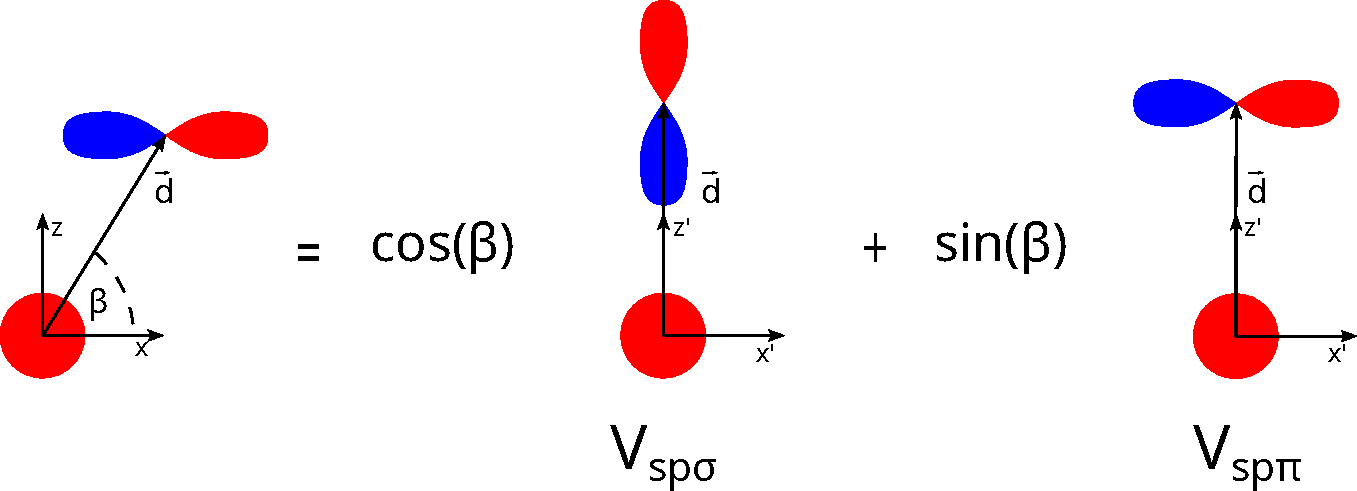
\includegraphics[width = \textwidth]{Plots/SK.pdf}
    \caption{Aufteilung eines allgemeinen $s$-$p$ Zweizentren-Integrals in die Integrale $V_{sp\sigma}$ und $V_{sp\pi}$ der zugehörigen Symmetrie.}
    \label{fig:TC}
\end{figure}
Dazu wird das $p_x$-Orbital in ein $p_z$- und ein $p_x$-Orbital zerlegt, wie in Abbildung \ref{fig:TC} zu sehen ist \cite{SC_literature, electronic_structure}.
Der Anteil der Bindung, ausgehend von dem $p_z$-Orbital, geht in das Integral $V_{sp\sigma}$ ein, während 
der Anteil von dem $p_x$-Orbital das Integral $V_{sp\pi}$ bildet.
Jedoch verschwindet das Integral $V_{sp\pi}$ in diesem Beispiel aufgrund der Symmetrie \cite{SC_literature}.
Im Allgemeinen sind die SK-Integrale \eqref{eqn:SK} durch die Zerlegung in die einzelnen Integrale $V_{ll'\eta}$ mit Vorfaktoren (siehe \cite{PhysRev.94.1498}),
den Richtungskosinus, gegeben \cite{SC_literature}.
Die Richtungskosinus 
\begin{equation}
    l = \frac{\vec{d} \cdot \hat{x}}{\left | \vec{d} \right |} \; , \quad
    m = \frac{\vec{d} \cdot \hat{y}}{\left | \vec{d} \right |} \; , \quad
    n = \frac{\vec{d} \cdot \hat{z}}{\left | \vec{d} \right |} \label{eqn:RK}
\end{equation}
sind die Projektionen des normierten Abstandsvektors auf die Einheitsvektoren $\hat{x}$, $\hat{y}$ und $\hat{z}$ \cite{SC_literature}.
Wurden diese bestimmt, können die Integrale $V_{ll'\eta}$ als z.B. Fitparameter oder empirische Werte fungieren. 
Werden die Orbital-Indizes vertauscht (z.B. $E_{z,xy} \to E_{xy, z}$), erhalten die Richtungskosinus ein negatives Vorzeichen, d.h. $(l,m,n) \to (-l,-m,-n)$ \cite{PhysRev.94.1498}.